\documentclass[a4paper]{article}
\usepackage[letterpaper, margin=1in]{geometry} % page format
\usepackage{listings} % this package is for including code
\usepackage{graphicx} % this package is for including figures
\usepackage{amsmath}  % this package is for math and matrices
\usepackage{amsfonts} % this package is for math fonts
\usepackage{tikz} % for drawings
\usepackage{hyperref} % for urls
\usepackage{pdfpages}

\title{Homework 0}
\author{Max Schemitsch}
\date{1/30/19}

\begin{document}
\lstset{language=Python}

\maketitle

\section{Python Requirements (2.1)}
\begin{lstlisting}[frame=single]
import sys
import numpy
import scipy
import sklearn
import matplotlib
import pandas
print(sys.version)
print(numpy.__version__ )
print(scipy.__version__) 
print(sklearn.__version__) 
print(matplotlib.__version__)
print(pandas.__version__)
\end{lstlisting}

\begin{lstlisting}
3.7.2
1.16.0
1.2.0
0.20.2
3.0.2
0.24.0
\end{lstlisting}

\section{GitHub Class Repository (2.2)}
My GitHub username is mschemitsch. Here's the link to my class repository:

\url{https://github.com/mschemitsch/MaxSchemitsch_DATA_440}

\begin{figure}[h]
  \begin{center}
    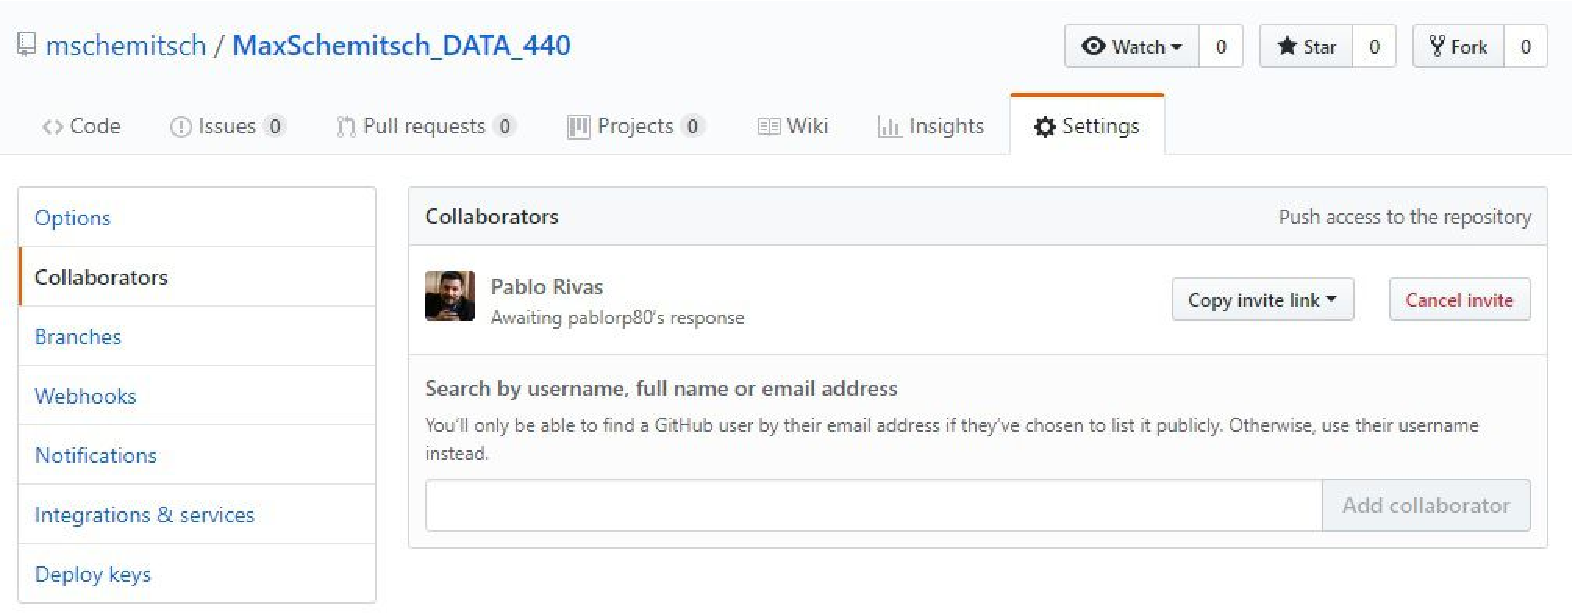
\includegraphics[width=0.75\textwidth]{github.pdf}
  \end{center}
\end{figure}


\section{Kaggle Account (2.3)}
My Kaggle username is mschemitsch.

\begin{figure}[h]
  \begin{center}
    
\includegraphics[width=0.75\textwidth]{kaggle.pdf}
  \end{center}
\end{figure}

\section{Problems}

\subsection{Question 1}
In order to find the value of $x$ that maximizes $g(x)=-3x^{2}+24x-30$, we must first take its derivative. We have that $g'(x)=-6x+24$. Then we evaluate the first derivative at 0. This gives us $x=4$. Thus $x=4$ maximizes $g(x)=-3x^{2}+24x-30$.

\subsection{Question 2}
In order to take the partial derivative of a function, we derive that parts we are respecting and treat the other parts as constants. The partial derivative of $f(x)=3x_{0}^{3}-2x_{0}x_{1}^{2}+4x_{1}-8$ with respect to $x_{0}$ is $9x_{0}^{2}-2x_{1}^{2}$. The partial derivative with respect to $x_{1}$ is $-4x_{0}x_{1}+4$.

\subsection{Question 3}
a)
\begin{lstlisting}[frame=single]
import numpy
A = numpy.array([[1, 4, -3], [2, -1, 3]])
B = numpy.array([[-2, 0, 5], [0, -1, 4]])
A.dot(B)
\end{lstlisting}
\begin{lstlisting}
Traceback (most recent call last):
   File “<stdin>”, line 1, in <module>
ValueError: shapes (2,3) and (2,3) not aligned: 3 (dim 1) != 2 (dim 0)
\end{lstlisting}

This error means that the two matrices are unable to be multiplied. This is because the dimensions don’t match for there to be a dot product. 2 by 3 matrices, like both A and B, can only be multiplied with a matrix of at least 3 rows. \\

b)
\begin{lstlisting}[frame=single]
A.T.dot(B)
numpy.linalg.matrix_rank(A.T.dot(B))
\end{lstlisting}

\begin{lstlisting}
array([[-2, -2, 13],
       [-8, 1, 16],
       [6, -3, -3]])
\end{lstlisting} \par

c)
\begin{lstlisting}[frame=single]
C=numpy.array([[1,0], [0,2]])
A.dot(B.T)+numpy.linalg.inv(C)
\end{lstlisting}

\begin{lstlisting}
array([[-16. , -16. ],
       [ 11. , 13.5]])

\end{lstlisting}

\subsection{Question 4}
A simple Gaussian, or normal distribution, has a probability density function of $\frac{1}{\sigma\sqrt{2\pi}}e^{-\frac{(x-\mu)^{2}}{2\sigma^{2}}}$ with $E[X]=\mu$ and $Var[X]=\sigma^{2}$. \par
A multivariate Gaussian distribution is similar to a simple Gaussian distribution, but utilizes more than one variable. Instead of being a 2 dimensional bell curve, it is instead a 3 dimensional curve. \par
A Bernoulli distribution, $X\mathtt{\sim}Bernoulli(p)$ utilizes a single probability $p$. Its probability mass function is $p$ if $k=1$ or $q=1-p$ if $k=0$. Its expected value is $p$ and variance is $pq$. \par
A binomial distribution utilizes a similar $p$ probability and also number of trials $n$. Its probability mass function is $\binom{n}{k}p^{k}(1-p)^{n-k}$. It has an expected value of $np$ and variance of $np(1-p)$. \par
An exponential distribution a rate of $\lambda$. Its probability density function is $\lambda e^{-\lambda x}$ and its cumulative distribution function is $1-e^{-\lambda x}$. It has an expected value of $\frac{1}{\lambda}$ and variance of $\frac{1}{\lambda ^{2}}$.

\subsection{Question 5}
The binomial distribution is a representation of how many successes occur in $n$ independent Bernoulli distribution experiments or trials.

\subsection{Question 6}
The expected value for $X \mathtt{\sim} N(2,3)$, a normal distribution with $ \mu = 2 $ and $ \sigma = 3$, is equal to its $ \mu $ or 2.

\subsection{Question 7}
a)
\begin{equation}
x^{*}=arg_{x} min||x-y||_{2}^{2}
\end{equation}

This equation represents that $x^{*}$ equals the $x$ value that minimizes the squared vector 2-norm of $x-y$. If $y=1.1$ and $Z=N$, $x^{*}$ is equal to the value that minimizes $||x-1.1||_{2}^{2}$ 

b)
\begin{figure}[h]
  \begin{center}
    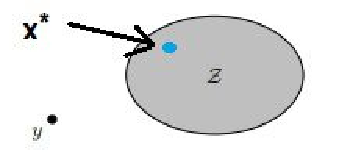
\includegraphics[height=8mm, width=20mm]{question7b.pdf}
  \end{center}
\end{figure}

\subsection{Question 8}
a) $\int_{-\infty}^{\infty} e^{-y}dy = -e^{-y}|_{0}^{\infty} = 1$ \\ \\
b) $E[Y] = \int_{0}^{\infty} ye^{-y}dy = e^{-y}(-y-1)|_{0}^{\infty} = 1$ \\ \\
c) $Var[Y] = \int_{0}^{\infty}(y-1)^{2}dy = \frac{y^{3}}{3}-y^{2}+y |_{0}^{\infty} = ???$ \\ \\
d) \\
Sorry, I couldn't quite figure out question D or the end of question C.

\end{document}
